\section{DENEYSEL ÇALIŞMALAR}

\begin{comment}
5. DENEYSEL ÇALIŞMALAR
5.1 Genel Bilgiler
Burada deneysel çalışmanın genel kapsamı, amacı ve yaklaşımı kısaca açıklanabilir.

Örneğin: “Bu bölümde, projede kullanılan sistemin fiziksel olarak nasıl kurulduğu, hangi yöntemlerle veri toplandığı ve deneylerin nasıl gerçekleştirileceği anlatılacaktır.”

Eğer henüz deney yöntemi kesinleşmediyse, planlanan deneysel çalışmaların genel hatlarından, amaçlarından ve beklenen sonuçlardan bahsedebilirsin.

5.2 Kurulum ve Sistem Tasarımı
Projende kullanılan sistemin (örneğin sensörler, donanım platformu, veri toplama düzeni) teknik özellikleri ve kurulum aşamaları detaylandırılabilir.

Bu kısımda varsa devre şemaları, bağlantı diyagramları ve sistemin fotoğrafları konulmalı.

Örneğin: “Sistemde kullanılan LDR sensörlerinin teknik özellikleri ve bunların bitkiye yerleştirilme şekli anlatılır.”

5.3 Veri Toplama ve Deneysel Prosedür
Deneylerin nasıl yapılacağı, hangi koşullarda veri toplanacağı (zamanlama, ortam koşulları vb.) açıklanmalı.

Projenin temelinde insan hareketi algılama varsa, bu hareketlerin deney ortamında nasıl gerçekleştirileceği veya simüle edileceği belirtilebilir.

Güvenlik önlemleri varsa, bu bölümde standartlara uygun olarak anlatılmalı.

5.4 Karşılaşılan Zorluklar ve Çözümler
Deney sırasında ortaya çıkabilecek ya da çıktıktan sonra yaşanan teknik problemler, bunların nasıl çözüldüğü, hangi kolaylıklar olduğu yazılabilir.

Örnek: “Bitkinin hassas yapısı nedeniyle sensörlerin konumlandırılması sırasında titreşim kaynaklı sinyal gürültüsü oluştu. Bu durum, … yöntemleriyle minimize edilmiştir.”

5.5 Testlerin Gerçekleştirilmesi
Tasarlanan sistemin çalışıp çalışmadığını test etmek için yapılacak testlerin türü, koşulları ve nasıl uygulanacağı anlatılmalı.

Eğer varsa test düzenekleri ve bağlantı şemaları bu alt başlıkta verilir.




\subsection{Genel Bilgiler}

\subsubsection{Deneyin Amacı ve Kapsamı}
Bu deneyin temel amacı, simülasyon ortamında elde edilen sonuçların fiziksel ortamda da doğrulanmasıdır. Bilgisayar ortamındaki ideal koşullardan farklı olarak gerçek dünyadaki değişkenlerin etkisi incelenir. Böylece modelin gerçek hayatta nasıl performans gösterdiği ortaya konur.

\subsubsection{Deneyin Gerçekleştirildiği Ortam}
Deney, kontrol edilen bir laboratuvar ortamında gerçekleştirilmiştir. Ortam ışık, sıcaklık gibi dış etkiler minimize edilerek deneyin sağlıklı ve tekrarlanabilir olması sağlanmıştır. Deney alanının fiziksel düzeni, kullanılan ekipmanların konumu ve yerleşimi detaylı olarak planlanmıştır.

\subsubsection{Kullanılan Ekipmanların Genel Tanıtımı}
Deneyde temel olarak ışığa duyarlı LDR sensörleri, veri toplama kartı ve sinyal işleme devreleri kullanılmıştır. Her bir ekipmanın teknik özellikleri ve çalışma prensipleri kısaca tanıtılmıştır. Bu sayede deneyin hangi bileşenler üzerinden yürütüldüğü anlaşılmaktadır.

\subsection{Deney Düzeneğinin Kurulumu ve Kullanımı}

\subsubsection{Sensör ve Ölçüm Elemanları}
LDR sensörleri ışık yoğunluğunu elektrik sinyaline dönüştürür ve deneyde bitkideki hareketi algılamak için kullanılır. Sensörlerin yerleşimi ve bağlantıları, ölçüm hassasiyetini artıracak şekilde tasarlanmıştır. Teknik özellikleri, çalışma voltajı ve tepki süreleri açıklanmıştır.

\subsubsection{Sinyal Koşullandırma ve Veri Toplama}
Sensörlerden gelen zayıf elektrik sinyalleri, sinyal koşullandırma devreleri ile uygun seviyeye getirilir. Veri toplama kartı bu sinyalleri dijital forma çevirerek bilgisayara aktarır. Bu süreçte sinyalin gürültüden arındırılması için filtreleme yapılmıştır.

\subsubsection{Yazılım ve Veri İşleme}
Gerçek zamanlı veri işleme için özel yazılım geliştirilmiştir. Yazılım, sensörlerden gelen verileri okuyarak hareket tespiti için makine öğrenmesi modeline gönderir. Kullanıcı arayüzü sayesinde deney anında veriler gözlemlenebilir ve kayıt altına alınabilir.

\subsubsection{Bağlantı Şemaları ve Fiziksel Düzen}
Deneyde kullanılan tüm elektronik bileşenlerin bağlantı şemaları detaylı şekilde çizilmiştir. Fiziksel yerleşim, bileşenlerin kolay erişilebilir ve güvenli olmasına dikkat edilerek planlanmıştır. Fotoğraflarla desteklenen bu bölümde deneyin kurulumu net olarak gösterilmektedir.

\subsection{Deney Sırasında Karşılaşılan Zorluklar ve Güvenlik Önlemleri}

\subsubsection{Ortam Koşullarından Kaynaklanan Zorluklar}
Deney ortamındaki ışık değişimleri ve sıcaklık dalgalanmaları ölçüm sonuçlarını etkileyebilmektedir. Bu tür dış etkenler için çeşitli önlemler alınmış, ortam kontrollü tutulmaya çalışılmıştır. Ancak tam izolasyon sağlanamadığından bu faktörlerin etkisi değerlendirilmiştir.

\subsubsection{Elektriksel ve Mekanik Güvenlik Önlemleri}
Deneyde kullanılan elektronik devrelerde kısa devre ve aşırı akım gibi risklere karşı koruyucu sigortalar ve devre kesiciler kullanılmıştır. Ayrıca cihazların mekanik yerleşiminde sağlamlık ve sabitleme ön planda tutulmuştur. Deney alanında yangın ve elektrik çarpması risklerine karşı gerekli uyarılar yapılmıştır.

\subsubsection{Kullanıcı Güvenliği ve İşaretlemeler}
Deney alanında kullanılan tüm ekipmanlar için uygun uyarı işaretleri yerleştirilmiştir. Kullanıcıların deney sırasında dikkat etmesi gereken güvenlik kuralları belirtilmiş ve eğitim verilmiştir. İşaretlemeler, potansiyel tehlikeleri açıkça göstermektedir.

\subsection{Deneyin Kullanımı ve Tekrarlanabilirliği}

\subsubsection{Kurulum Talimatları}
Deneyin kurulumu için adım adım uygulanması gereken işlemler detaylı olarak açıklanmıştır. Ekipmanların bağlanması, sensör yerleşimi ve yazılımın kurulumu gibi aşamalar kullanıcıya rehberlik edecek şekilde sunulmuştur. Bu sayede deney kolaylıkla tekrarlanabilir.

\subsubsection{Deney Prosedürleri}
Deney sürecinde izlenecek adımlar, ölçüm alınması ve veri kaydı prosedürleri sistematik biçimde anlatılmıştır. Deney sırasında dikkat edilmesi gereken noktalar ve gözlemlenecek parametreler belirtilmiştir. Böylece tutarlı ve doğru veri elde edilmesi sağlanır.

\subsubsection{Veri Kaydı ve Analiz İçin Gerekenler}
Toplanan verilerin kaydedilmesi, depolanması ve analiz için hazırlanması aşamaları açıklanmıştır. Veri formatları ve kullanılacak analiz araçları hakkında bilgi verilmiştir. Bu bilgiler, deney sonuçlarının daha sonra doğrulanmasını kolaylaştırır.

\subsubsection{Tekrarlanabilirlik ve Kullanıcı Rehberi}
Deneyin farklı kişiler tarafından benzer koşullarda tekrarlanabilmesi için gerekli öneriler ve uyarılar sunulmuştur. Kurulum ve ölçümde dikkat edilmesi gereken önemli noktalar vurgulanmıştır. Bu sayede deneyin güvenilirliği ve geçerliliği artırılmıştır.


\end{comment}


\subsection{Genel Bilgiler}
Bu bölümde, STM32H723ZTG6U mikrodenetleyicisi üzerinde geliştirilen sistemin deneysel çalışmaları detaylandırılmıştır. Projede, pasif bir devre elemanı olan LDR (Işık Bağımlı Direnç) sensörü kullanılarak, üzerinde eğitilmiş derin öğrenme modeli ile düşük maliyetli ve taşınabilir bir akıllı algılayıcı prototipi oluşturulmuştur. 

Deney kapsamında, geliştirilen model CubeIDE entegre geliştirme ortamı kullanılarak mikrodenetleyiciye yüklenmiş ve gerçek zamanlı veri okuma ile işleme fonksiyonları başarıyla gerçekleştirilmiştir. Ayrıca, projemizde deney kutusu kullanılmış ve sistem önünden her biri üç farklı kişi tarafından 100'er defa geçilerek veri toplama işlemi tamamlanmıştır.


\begin{figure}[H]
    \centering
    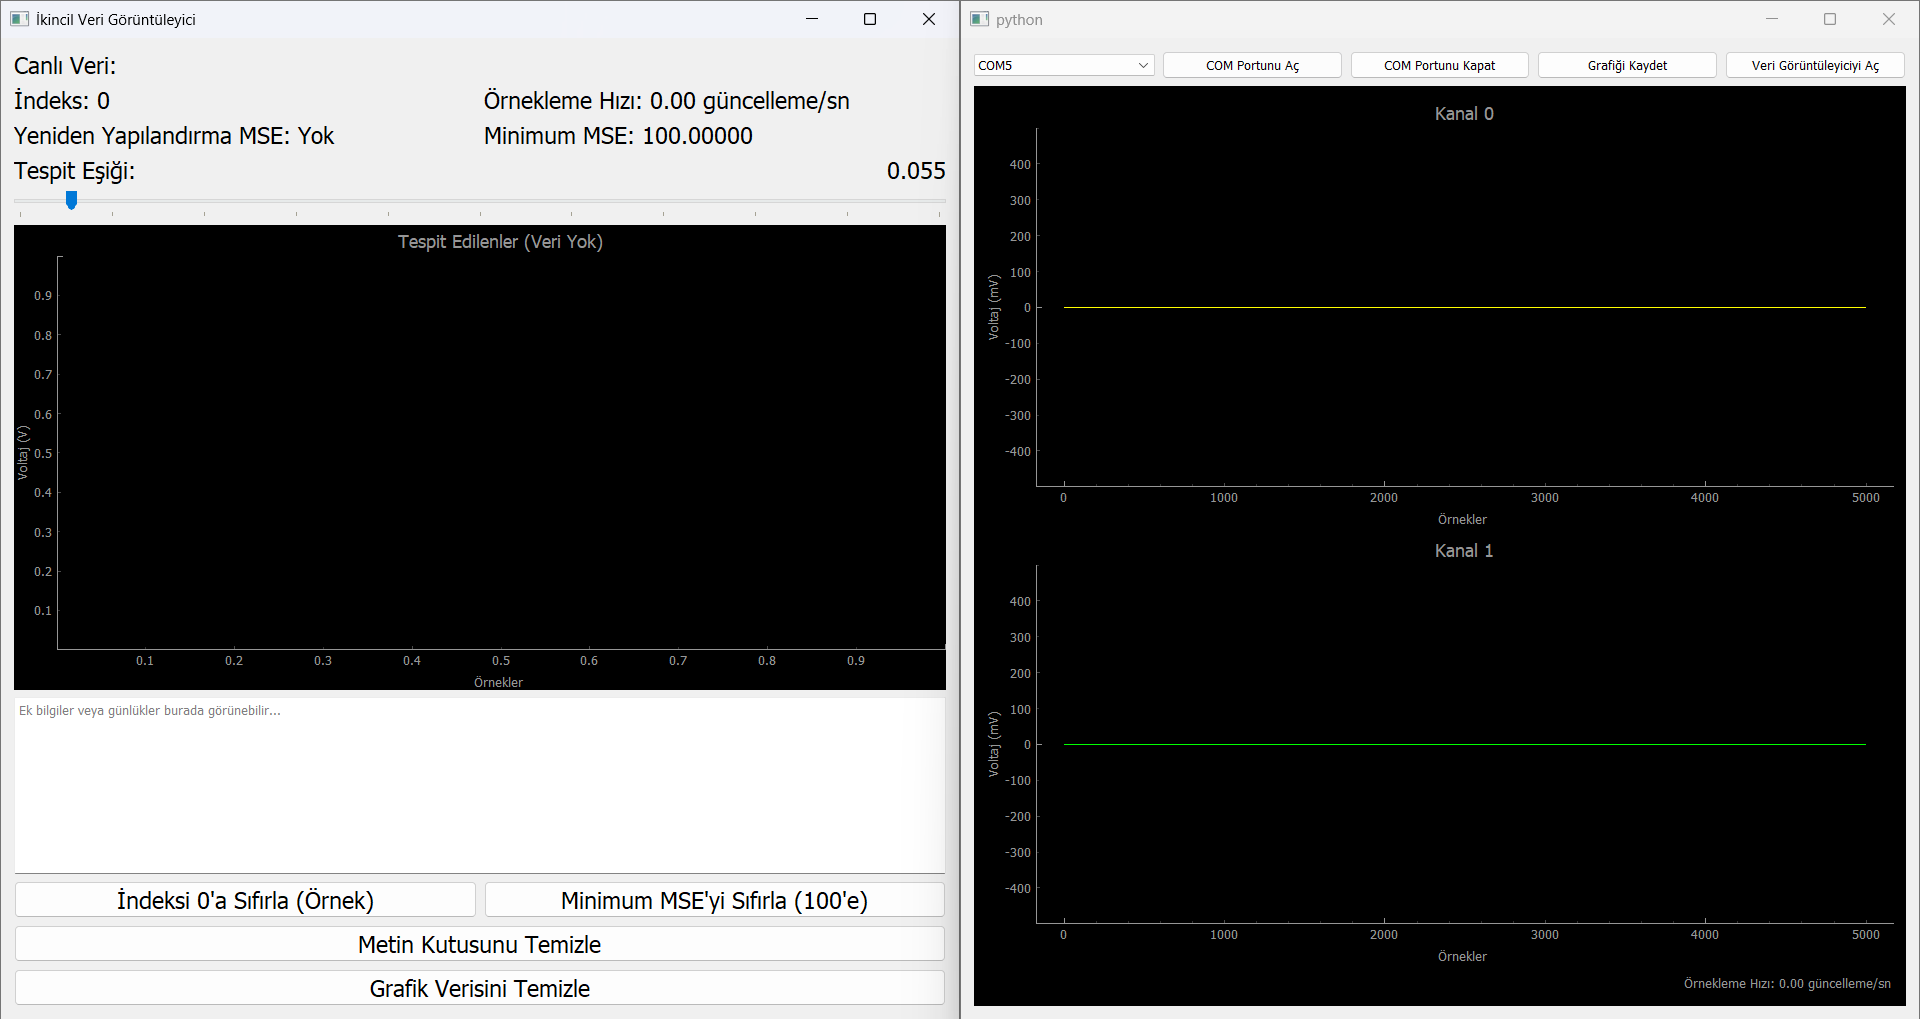
\includegraphics[width=1\linewidth]{image_deney.png}
    \caption{Deneyde kullanılan veri gönderim ve izleme arayüzü programı}
    \label{fig:deney_arayuz}
\end{figure}

\newpage

Sistemden gönderilen verilerin takibi için Python dili ile geliştirilmiş bir arayüz programı yazılmıştır. Bu program, deney verilerinin anlık izlenmesini sağlamış ve deneyin doğru şekilde yürütülmesine olanak tanımıştır. Bu program \ref{fig:deney_arayuz}de görülmektedir. Deney düzeneği \ref{fig:deney_kutu}deki gibidir

\begin{figure}[H]
    \centering
    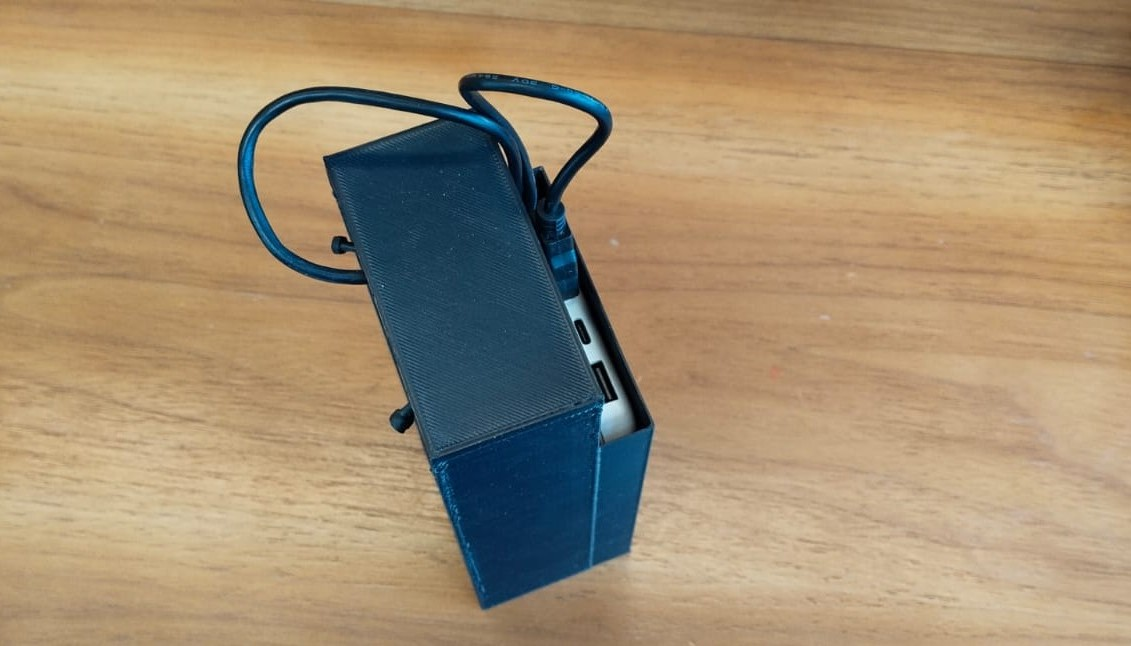
\includegraphics[width=0.75\linewidth]{media/deney_kutu1.jpg}
    \caption{Deney Düzeneği}
    \label{fig:deney_kutu}
\end{figure}



\subsection{Arayüz Elemanlarının Gerçeklenmesi}
Deneyde temel arayüz, STM32H723ZTG6U mikrodenetleyicisi ile LDR sensörü arasında kurulmuştur. Mikrodenetleyici, LDR’den aldığı analog sinyali ADC modülü aracılığıyla dijital forma dönüştürmüş ve bu veriler derin öğrenme modeline giriş olarak kullanılmıştır.

Bluetooth modülü deneyde veri iletimi için sisteme entegre edilmiş ve başarılı bir şekilde çalıştırılarak verilerin uzak bir bilgisayara aktarımı sağlanmıştır. Bu sayede, gerçek zamanlı veri izleme ve kayıt işlemleri mümkün hale gelmiştir.

Kullanılan LDR sensörünün teknik özellikleri arasında düşük maliyetli, pasif yapıda olması ve çevresel ışık değişimlerine duyarlı ölçümler yapabilmesi yer almaktadır. Sensörün karakteristik eğrisi, ışık şiddeti arttıkça direncinin azaldığını göstermektedir; bu da ADC aracılığıyla mikrodenetleyicide okunabilmesini sağlamıştır.

\subsection{Yapılan Testler}
Sistem üzerinde gerçekleştirilen testler, sensör verilerinin doğruluğunu ve derin öğrenme modelinin mikrodenetleyicide etkin çalışmasını doğrulamaya yönelik olmuştur. Her üç kişi deney kutusunun önünden 100'er kez geçerek veri toplanmış ve bu veriler Python arayüzü ile başarıyla görüntülenmiştir.

Testlerde, sistemin ışık koşullarına verdiği tepki ve sensör verilerinin doğru şekilde işlenmesi gözlemlenmiştir. Bluetooth haberleşmesindeki stabilite ve veri iletim başarısı test edilmiş, güvenilir ve gerçek zamanlı veri aktarımı sağlanmıştır.

Deney sırasında ışık ortamı, sensör yerleşimi ve mikrodenetleyicinin çalışma kararlılığı gibi koşullar titizlikle kontrol edilmiştir. Test sonuçları, sistemin tasarım amaçlarına uygun şekilde çalıştığını göstermiştir.

Deney düzeneğinin bağlantı şeması ve baskı devre çizimleri raporun ilgili bölümlerinde verilmiştir.

